\chapter{Utilities}
\label{ch:utilities}

The functionalities shared between all the components of LAR
are defined in here.

@O lib/jl/utilities.jl
@{@< Aliases @>
@< Utilities @>
@}

\subsection{Tests}
As usual every function has some unit tests.

@O test/jl/utilities.jl
@{using Base.Test
include("../../lib/jl/utilities.jl")

@< Utilities tests @>
@}


%%%%%%%%%%%%%%%
\section{Types}

To store vertices and cells boundary matrices, 
we use types already built in the standard Julia.
We use these aliases to standardize the types used 
throughout LAR. 

@D Aliases
@{const Verts = Array{Float64, 2}
const Cells = SparseMatrixCSC{Int8, Int}
const Cell = SparseVector{Int8, Int}
@}




%%%%%%%%%%%%%%%%%%%%%%%%
\section{Bounding boxes}
\label{sec:bboxes}

Bounding boxes are essential in many steps of many
algorithms in LAR. Here we present a method for building
and performing containment tests on n-dimensional bounding boxes.

@D Utilities
@{function bbox(vertices::Verts)
    minimum = mapslices(x->min(x...), vertices, 1)
    maximum = mapslices(x->max(x...), vertices, 1)
    minimum, maximum
end

function bbox_contains(container, contained)
    b1_min, b1_max = container
    b2_min, b2_max = contained
    all(map((i,j,k,l)->i<=j<=k<=l, b1_min, b2_min, b2_max, b1_max))
end
@}

\subsection{Tests}
\begin{figure}[h]
    \centering
    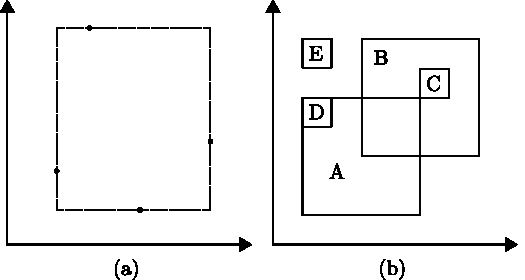
\includegraphics{./img/ch5-bboxes.pdf}
    \caption{(a) is a visualization of the test for bboxes building, (b) for bbox containment.}
\end{figure}
@D Utilities tests
@{@@testset "Bounding boxes building test" begin
    V = [.56 .28; .84 .57; .35  1.0; .22  .43]
    @@test bbox(V) == ([.22 .28], [.84 1.0])
end

@@testset "Bounding boxes containment test" begin
    bboxA = ([0. 0.], [1. 1.])
    bboxB = ([.5 .5], [1.5 1.5])
    bboxC = ([1. 1.], [1.25 1.25])
    bboxD = ([0 .75], [.25 1])
    bboxE = ([0 1.25], [.25 1.5])

    @@test bbox_contains(bboxA, bboxD)
    @@test bbox_contains(bboxB, bboxC)
    @@test !bbox_contains(bboxA, bboxB)
    @@test !bbox_contains(bboxA, bboxE)
end
@}

%%%%%%%%%%%%%%%%%%%%%%%%%%%%%%%
\section{Face area calculation}
\label{sec:face_area}

\begin{figure}[h]
    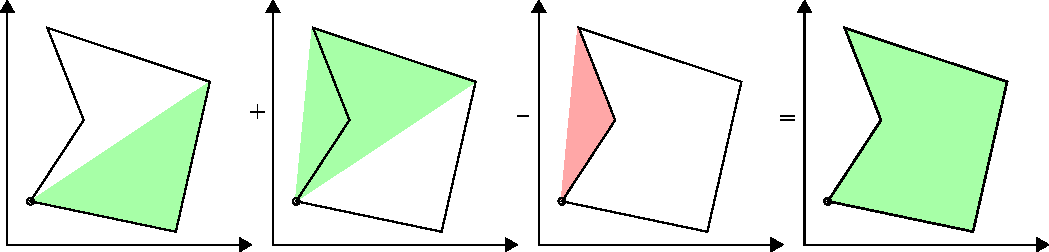
\includegraphics[width=\textwidth]{./img/ch5-area.pdf}
    \caption{A visual representation of the face area calculation algorithm. The area
    of the face is the sum of the areas of each triangle which can be build using the 
    pivot vertex and the other vertices of the face}
\end{figure}
\noindent
To compute the area of a generic (convex or concave) face,
we pick a pivot vertex of the face and then we iterate over
every edge of the face calculating the area of the triangle
made by the pivot vertex and the ordered extremes of the current edge.
The area of the full face is the sum of the areas of the single triangles.
This works because of the single triangles we compute the signed area with
this formula:
\begin{gather*}
    A = \frac{1}{2}
    \begin{vmatrix}
        p_{1x} & p_{1y} & 1 \\
        p_{2x} & p_{2y} & 1 \\
        p_{3x} & p_{3y} & 1
    \end{vmatrix}
\end{gather*}
Where $p_1$, $p_2$ and $p_3$ are the vertices of the triangle ($p_1$ is the pivot vertex). 
Please notice that the result of this formula will be negative only if these vertices 
are arranged in clockwise order.

@D Utilities
@{function face_area(V::Verts, EV::Cells, face::Cell)
    function triangle_area(triangle_points::Verts)
        ret = ones(3,3)
        ret[:, 1:2] = triangle_points
        return .5*det(ret)
    end

    area = 0
    ps = [0, 0, 0]

    for i in face.nzind
        edge = face[i]*EV[i, :]
        skip = false

        for e in edge.nzind
            if e != ps[1]
                if edge[e] < 0
                    if ps[1] == 0
                        ps[1] = e
                        skip = true
                    else
                        ps[2] = e
                    end
                else
                    ps[3] = e
                end
            else
                skip = true
                break
            end
        end

        if !skip
            area += triangle_area(V[ps, :])
        end
    end

    return area
end
@}

\subsection{Tests}
\begin{figure}[h]
    \centering
    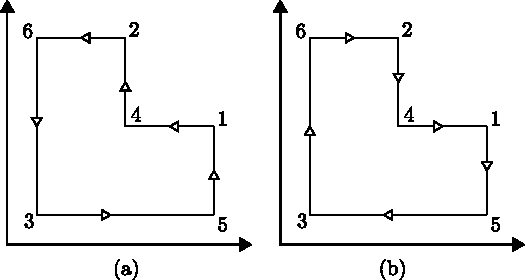
\includegraphics{./img/ch5-area_test.pdf}
\end{figure}
\noindent The two faces drawn above they must have complimentary area.
@D Utilities tests
@{@@testset "Face area calculation test" begin
    V = Float64[2 1; 1 2; 0 0; 1 1; 2 0; 0 2]
    EV = spzeros(Int8, 6, 6)
    EV[1, [1, 4]] = [-1, 1]; EV[2, [2, 4]] = [-1, 1]
    EV[3, [2, 6]] = [-1, 1]; EV[4, [3, 6]] = [-1, 1]
    EV[5, [3, 5]] = [-1, 1]; EV[6, [1, 5]] = [-1, 1]
    FE = spzeros(Int8, 2, 6)
    FE[1, :] = [ 1 -1  1 -1  1 -1]
    FE[2, :] = [-1  1 -1  1 -1  1]

    @@test face_area(V, EV, FE[1,:]) == -face_area(V, EV, FE[2,:])
end
@}

%%%%%%%%%%%%%%%%%%%%%%%%
\section{Skeletal merge}

It is generally useful to have a utility to merge the skeletons of
two cellular complexes. We have both the $d=2$ and $d=3$ versions.

@D Utilities
@{function skel_merge(V1::Verts, EV1::Cells, V2::Verts, EV2::Cells)
    V = [V1; V2]
    EV = spzeros(Int8, EV1.m + EV2.m, EV1.n + EV2.n)
    EV[1:EV1.m, 1:EV1.n] = EV1
    EV[EV1.m+1:end, EV1.n+1:end] = EV2
    V, EV
end

function skel_merge(V1::Verts, EV1::Cells, FE1::Cells, V2::Verts, EV2::Cells, FE2::Cells)
    FE = spzeros(Int8, FE1.m + FE2.m, FE1.n + FE2.n)
    FE[1:FE1.m, 1:FE1.n] = FE1
    FE[FE1.m+1:end, FE1.n+1:end] = FE2
    V, EV = skel_merge(V1, EV1, V2, EV2)
    V, EV, FE
end
@}

%%%%%%%%%%%%%%%%%%%%%%
\section{Point in face area}
\label{sec:point_in_face}

One correct way to check if a point lays in the area of a general 2D face
is to shoot a ray from that point with the same direction
of the positive $x_1$ semi-axis and then count the intersection found
with the edges of the face.

The math behind this procedure is explained here:
First of all we parametrize the edge made of the $p_1$ and $p_2$ points:

\begin{equation}
\label{eq:edge}
    p = p_1 + \alpha(p_2-p_1), \quad\alpha\in[0, 1]
\end{equation}

Then we find the value that $\alpha$ assumes when the edge
intersects the line parallel to the $x_1$ axis that passes through $o$,
the point of which we need to check the inclusion inside the face:

\begin{gather*}
    \begin{bmatrix}
        o_x \\ o_y
    \end{bmatrix}
    = 
    \begin{bmatrix}
        p_{1x} \\ p_{1y}
    \end{bmatrix}
    +
    \alpha
    \begin{bmatrix}
        p_{2x} - p_{1x} \\ p_{2y} - p_{1y}
    \end{bmatrix} \\
    o_y = p_{1y} + \alpha(p_{2y} - p_{1y}) \\
    \alpha = \frac{o_y - p_{1y}}{p_{2y} - p_{1y}}
\end{gather*}

If $\alpha\in[0, 1]$ then the edge intersect the line, and we find the point
of intersection by putting $\alpha$ into equation \ref{eq:edge}.
The intersection must be count only if the freshly computed point
is on the right of $o$.

In the implementation, additional care is needed when the ray encounters a vertex
(or, mathematically speaking, when $\alpha\in\{0, 1\}$):
we are testing the intersections of the ray with edges, and every
vertex is shared by two or more edges. So we cannot simply increase the 
\texttt{hits} counter every time we encounter a vertex because this will lead
to miscalculations when an even number of edges share the same vertex.
We resolve this by storing the already visited vertices into the 
\texttt{visited\_verts} list.

@D Utilities
@{function point_in_face(origin, V::Verts, ev::Cells)
    hits = 0
    visited_verts = []

    for edge in 1:ev.m
        a_id, b_id = ev[edge, :].nzind
        a = V[a_id, :]
        b = V[b_id, :]
        v = b - a
        alpha = (origin[2] - a[2]) / v[2]
        if 0 <= alpha <= 1
            x_int = a[1] + v[1]*alpha
            if x_int > origin[1]
                if 0 < alpha < 1
                    hits += 1
                else
                    p = (alpha == 0) ? a : b
                    if !(p in visited_verts)
                        hits += 1
                        push!(visited_verts, p)
                    end
                end
            end
        end
    end

    return hits % 2 == 1
end
@}

%%%%%%%%%%%%%%%%%%%%%%%
\section{Edge deletion}
\label{sec:delete_edges}

Deleting edges ia a common operation in planar arrangement. When
edges are deleted, some vertices can remain unconnected; these must be deleted too.

@D Utilities
@{function delete_edges(todel, V::Verts, EV::Cells)
    tokeep = setdiff(collect(1:EV.m), todel)
    EV = EV[tokeep, :]
    
    vertinds = 1:EV.n
    todel = Array{Int64, 1}()
    for i in vertinds
        if length(EV[:, i].nzind) == 0
            push!(todel, i)
        end
    end

    tokeep = setdiff(vertinds, todel)
    EV = EV[:, tokeep]
    V = V[tokeep, :]

    return V, EV
end
@}


%%%%%%%%%%%%%%%%%%%%%%%
\section{FV building}

Sometimes is useful to represent a face like a sequence of vertices.

@D Utilities
@{function buildFV(EV::Cells, face::Cell)
    startv = -1
    nextv = 0
    edge = 0

    vs = []

    while startv != nextv
        if startv < 0
            edge = face.nzind[1]
            startv = EV[edge,:].nzind[face[edge] < 0 ? 2 : 1]
            push!(vs, startv)
        else
            edge = setdiff(intersect(face.nzind, EV[:, nextv].nzind), edge)[1]
        end
        nextv = EV[edge,:].nzind[face[edge] < 0 ? 1 : 2]
        push!(vs, nextv)

    end

    return vs[1:end-1]
end
@}



%%%%%%%%%%%%%%%%%%%%%
\section{Vertex equality utilities}

@D Utilities
@{function vin(vertex, vertices_set)
    for v in vertices_set
        if vequals(vertex, v)
            return true
        end
    end
    return false
end

function vequals(v1, v2)
    err = 10e-8
    return length(v1) == length(v2) && all(map((x1, x2)->-err < x1-x2 < err, v1, v2))
end
@}